\section{Introduction}


%Repeat what was in the intro a bit

%Why do this?

%say something about \texttt{mmds}

%Do I need to say something about Len here?


%%%%%%%%%%%%%%%%%%%%%%%%%%%%%%%%%%%%%%%%%%%%%%%%%%%
\section{General formulation}

This section lays out a mixture model formulation for distance sampling detection functions. Beginning with the simplest case (line transects with no covariates) the models are built up and it is shown that the simpler models are just special cases of the more complex ones, thus providing a general framework for mixture model detection functions.

The core principle here is to replace the ``key function plus adjustment terms'' model for the detection function with a mixture model. The simplest example would be to define the detection function, $g$, as some finite weighted sum of half-Normal distributions:
\begin{equation}
g(x;\bm{\sigma},\bm{\pi}) = \sum_{j=1}^J \pi_j \exp \Big( \frac{-x^2}{2 \sigma_j^2}\Big).
\label{mmds-simplemix}
\end{equation}
Where the mixture proportions, $\pi_j$, have the property $\sum_{\forall j}\pi_j=1$ and $\bm{\pi} = (\pi_1, \dots, \pi_J)$. $\bm{\sigma}=(\sigma_1,\sigma_2,\dots,\sigma_J)$ are scale parameters. An example of a 2-point mixture of half-Normals is given in figure \ref{2ptdia}.

TKTKTK physical explanation of models - interpretation as smooths curves vs. interpretation as sub-populations.

\begin{figure}
\centering
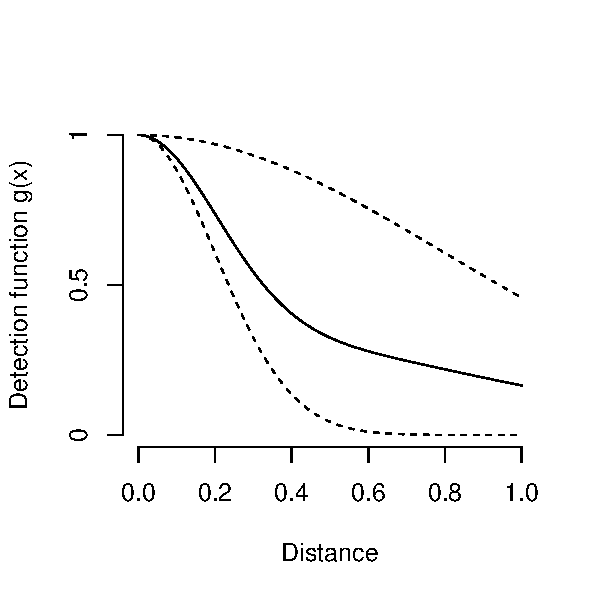
\includegraphics[width=3in]{mix/figs/2ptdia.pdf}
\caption{An example of a 2-point mixture of half-Normals. The two constituent mixture components are shown with dashed lines, the whole mixture function is the solid line. The scale parameters are $0.8$ and $0.2$. The associated mixture proportions are $0.64$ and $0.36$.}
\label{2ptdia}
\end{figure}

Clearly one can think of many variations on this theme: alternative functions, different functions for each mixture component, continuous mixtures or a finite mixture of continuous and finite mixtures (\textit{a la} \cite{morgan08}). However, here only finite mixtures of half-Normals are considered.

\subsection{Line transects}
For line transects, we can simply substitute equation (\ref{mmds-simplemix}) into the line transect likelihood in equation (\ref{ds-lt-likelihood}). Before doing this we first note that the definition of $\mu$ has not changed, merely the definition of $g$. Denoting $g_j$ as one of the component detection functions of the mixture,
\begin{align*}
\mu = \int_0^w \sum_{j=1}^J \pi_j g_j(x;\sigma_j) \text{d}x = \sum_{j=1}^J \pi_j \int_0^w  g_j(x;\sigma_j) \text{d}x = \sum_{j=1}^J \pi_j \mu_j.
\end{align*}
So, the likelihood is:
\begin{align}
\mathcal{L}(\bm{\sigma}, \bm{\pi}; \bm{x}) &= \prod_{i=1}^n f(x_i;\bm{\sigma}, \bm{\pi}),\\
&= \prod_{i=1}^n \frac{g(x_i;\bm{\sigma}, \bm{\pi})}{\mu},\\
&= \prod_{i=1}^n \frac{\sum_{j=1}^J \pi_j g_j(x_i;\sigma_j)}{\sum_{j=1}^J \pi_j \int_0^w  g_j(x;\sigma_j) \text{d}x},\\
&= \prod_{i=1}^n \sum_{j=1}^J \pi_j \frac{\exp \Big( \frac{-x_i^2}{2 \sigma_j^2}\Big)}{\int_0^w \exp \Big( \frac{-x_i^2}{2 \sigma_j^2}\Big) \text{d}x}.
\label{mmds-lt-likelihood}
\end{align}


Rather than decomposing $g$ into its constituent $g_j$s, the likelihood can be thought of as a mixture of PDF components, $f_j$, yielding the same final expression:
\begin{align}
\mathcal{L}(\bm{\sigma}, \bm{\pi}; \bm{x}) &= \prod_{i=1}^n f(x_i;\bm{\sigma}, \bm{\pi}),\\
&= \prod_{i=1}^n \sum_{j=1}^J \pi_j f_j(x_i;\bm{\sigma}, \bm{\pi}),\\
&= \prod_{i=1}^n \sum_{j=1}^J \pi_j \frac{\exp \Big( \frac{-x_i^2}{2 \sigma_j^2}\Big)}{\int_0^w  \exp \Big( \frac{-x_i^2}{2 \sigma_j^2}\Big) \text{d}x}.
\label{mmds-lt-likelihood-pdf}
\end{align}

\subsection{Point transects}
The detection function is, of course, the same for point transects as for line transects. What changes is the PDF and hence likelihood. The likelihood is therefore:
\begin{align}
\mathcal{L}(\bm{\sigma}, \bm{\pi}; \bm{r}) &= \prod_{i=1}^n f(r_i;\bm{\sigma}, \bm{\pi}),\\
&= \prod_{i=1}^n \sum_{j=1}^J \pi_j f_j(r_i; \sigma_j),\\
&= \prod_{i=1}^n \sum_{j=1}^J \pi_j \frac{g_j(r_i; \sigma_j,)}{\nu_j},\\
&= \prod_{i=1}^n \sum_{j=1}^J \pi_j \frac{r_i \exp \Big( \frac{-r_i^2}{2 \sigma_j^2}\Big)}{\int_0^w r  \exp \Big( \frac{-r_i^2}{2 \sigma_j^2}\Big) \text{d}r}.
\label{mmds-pt-likelihood-pdf}
\end{align}
where we can define a per-mixture effective area of detection:
\begin{equation}
\nu_j= 2 \pi \int_0^w r  g_j(r;\sigma_j) \text{d}r,
\end{equation}
which is analogous to $\mu_j$, above, and an overall area of detection:
\begin{equation}
\nu= \sum_{j=1}^J \pi_j \nu_j.
\end{equation}


Having these two likelihoods written down, the formulation for covariate models and the generalised likelihood can be derived.

\subsection{Covariate models}
The above models show that the differences between the CDS and mixture model DS (MMDS) are fairly minimal. For the covariate case things are a little more tricky. There are many possible model formulations and the notation is therefore more complicated.

Consider the case where one distance, $x$ (alternatively $r$ for point transects), has been observed and a set of corresponding covariates $z_1,\dots,z_K$ have been recorded too. As in MCDS the scale function is thought of as a (link) function of these covariates and a set of coefficients, the detection function is then defined as:
\begin{equation*}
g(x, \bm{z};\bm{\beta},\bm{\pi}) = \sum_{j=1}^J \pi_j \exp \Big( \frac{-x^2}{2 \sigma_j(\bm{z};\bm{\beta}_j)^2}\Big),
\label{mmds-detfct-covar}
\end{equation*}
and the scale parameter per mixture is defined as:
\begin{equation*}
\sigma_j(\bm{z};\bm{\beta}_j) = \exp \Big(\beta_{0j} + \sum_{k\in K_j} \beta_{kj} z_k \Big),
\end{equation*}
where $\bm{z}$ is the $K$-vector of all covariates. $K_j$ is the set of covariates to be used with mixture $j$. The vector of per mixture coefficients is $\bm{\beta}_j=(\beta_{0j},\{ \beta_{kj} : k \in K_j\})$. Finally $\bm{\beta}=(\bm{\beta}_1,\dots,\bm{\beta}_J)$ is the vector of all coefficients ordered by mixture part then covariate.

When we have multiple observations we store the distances in $\bm{x}$ (an $n$-vector). Then, for each observation we have a $\bm{z}_i$, which is a vector of covariates for that particular observation. $Z$ is an $n \cross K$ matrix of all covariates ie. the $\bm{z}_i$s stacked on top of each other. So then $z_{ik}$ would be the $i^\text{th}$ observation's covariate $k$ (and the $ik^\text{th}$ element of $Z$).

TKTKTK more here

%\subsubsection{Covariates - intercept model}
%
%One can think of a special case of the model above when the parameters estimated are common across all mixture components, except for an intercept.  Mathematically,
%\begin{align*}
%\sigma_j(\bm{z};\bm{\beta}_j) = \exp \Big(\beta_{0j} + \sum_{k\in K_j} \beta_{k} z_k \Big)
%\end{align*}
%so the $\beta_{0j}$s are estimated in each mixture but the $\beta_{k}$s are common to all mixtures and are estimated simultaneously. In this case, the $K_j$s are the same for all mixture components.
%
%NOT CURRENTLY IMPLEMENTED

\subsection{Generalised likelihood}
\label{ds-genlik}

\subsubsection{Line transects}
Considering the non-covariate case as a special case of the covariate model, the likelihood can then be written as:
\begin{align}
\mathcal{L}(\bm{\beta}, \bm{\pi} ; \bm{x}, Z) &= \prod_{i=1}^n f(x_i;\bm{\sigma}(\bm{z}_i, \bm{\beta})),\\
&= \prod_{i=1}^n \frac{g(x_i;\bm{\sigma}(\bm{z}_i, \bm{\beta}))}{\mu(\bm{z}_i)},\\
&= \prod_{i=1}^n \sum_{j=1}^J \pi_j \frac{g_j(x_i; \sigma_j(\bm{z}_i;\bm{\beta}_j))}{ \mu_j(\bm{z}_i)}.
\label{mmds-lt-glikelihood}
\end{align}
where $\mu(\bm{z}_i)$ is the sum of the $\mu_j$s per observation, i.e.
\begin{equation}
\mu(\bm{z}_i) = \sum_{j=1}^J \pi_j \int_0^w g_j(x; \sigma_j(\bm{z}_i;\bm{\beta}_j)) \text{d}x.
\end{equation}
where the $\sigma_j(\bm{z}_i;\bm{\beta}_j)$s take the covariate form above; in the case of a no covariate model, there is only the intercept term, $\beta_{0j}$ ie:
\begin{equation}
\sigma_j = \exp ( \beta_{0j} ).
\end{equation}

\subsubsection{Point transects}
For point transects the likelihood is similar, though with the $r$ pre-multiplier as seen for CDS and MCDS:
\begin{align}
\mathcal{L}(\bm{\beta}, \bm{\pi} ; \bm{r}, Z) &= \prod_{i=1}^n f(r_i;\bm{\sigma}(\bm{z}_i, \bm{\beta})),\\
&= \prod_{i=1}^n \frac{g(r_i;\bm{\sigma}(\bm{z}_i, \bm{\beta}))}{\nu(\bm{z}_i)},\\
&= \prod_{i=1}^n \sum_{j=1}^J \pi_j \frac{g_j(r_i; \sigma_j(\bm{z}_i;\bm{\beta}_j))}{ \nu_j(\bm{z}_i)}.
\label{mmds-pt-glikelihood}
\end{align}
So,
\begin{equation}
\nu(\bm{z}_i) = 2 \pi \sum_{j=1}^J \pi_j \int_0^w r g_j(r; \sigma_j(\bm{z}_i;\bm{\beta}_j)) \text{d}r.
\end{equation}


\subsection{Probability of detection}

(TKTKTK write more here!)

The detection probability, as we have seen, is a central concept in distance sampling. Notably, it can be used as a way of estimating abundance (via Horvitz-Thompson estimators). In this vein, the per-observation detectability is first derived. Next, an estimate of overall average detectability is often useful (and will be used later to asses the performance of the method), so this is also derived. Finally, the variance of the average detectability is also found and as a result of this, an estimator of the coefficient of variation is also given.

\subsubsection{Per-observation detectability}
When using covariates, each object effectively has its own detection function and hence its own per observation detectability. Calculating this is fairly simple. Starting from the definition of detectability given in equation (3.19) of Buckland \textit{et al} (2004) p 38 (modified slightly for notational consistency), the detection function is replaced with (\ref{mmds-detfct-covar}):
\begin{align*}
P_a(\bm{z}_i) =& \frac{\mu(\bm{z}_i)}{w},\\
=& \frac{1}{w} \int_0^w g(x; \sigma(\bm{z}_i,\bm{\beta})) \text{d}x,\\
=& \frac{1}{w} \int_0^w \sum_{j=1}^J \pi_j g_j(x; \sigma_j(\bm{z}_i, \bm{\beta}_j)) \text{d}x,\\
=& \frac{1}{w} \sum_{j=1}^J \pi_j \int_0^w  g_j(x; \sigma_j(\bm{z}_i, \bm{\beta}_j)) \text{d}x,
\end{align*}
so the detectability can now be calculated for each observation.


\subsubsection{Average detectability}
(TKTKTK  Fill this in!)

\subsubsection{Variance of $p$}

\subsubsection{CV}

\subsection{Goodness of fit testing}





%%%%%%%%%%%%%%%%%%%%%%%%%%%%%%%%%%%%%%%%%%%%%%%%%%%
\section{Implementation}
This section gives detail on the implementation of MMDS, particularly those used in the \textsf{R} package \texttt{mmds}.

(TKTKTK more here)

\subsection{Parametrisation of the scale parameters}
The parametrisation of the $\sigma_j$s given in section \ref{ds-genlik} is not only useful because it simplifies the notation in the likelihood. It also allows for unconstrained optimisation of the scale parameters in all situations. Since $\sigma_j$ must be positive, optimising a set of $\bm{\beta}_j$s on the log scale allows for the $\bm{\beta}_j$s to take values over all of $\mathbb{R}$.


\subsection{Parametrisation of the mixture proportions}
When using 2-point mixtures, the constraint that the $\pi_j$s must sum to unity is enforced by definition (since $\pi_2=1-\pi_1$). However, in $J$-point mixtures when $J>2$, ensuring that the proportions sum to 1 is not guaranteed. The obvious way to get around this would be to penalise the likelihood, should the optimisation procedure propose values for the $\pi_j$s that are not in accordance with this condition. This is, of course, inefficient and ugly. Instead, a parametrisation is used for the mixture proportions which yields $\pi_j$s that comply.

Rather than estimating the $\pi_j$s, estimate $\alpha_k$s, where the relationship between the two is:
\begin{equation*}
\pi_j = F(\sum_{k=1}^j e^{\alpha_k}) - F(\sum_{k=1}^{j-1} e^{\alpha_k}) \qquad \text{for } 1\leq j \leq J-1
\end{equation*}
and
\begin{equation*}
\pi_J = 1-\sum_{j=1}^{J-1} \pi_j
\end{equation*}
where $F$ is any continuous CDF on $(0,\infty]$. Exponentiation ensures that $e^{\alpha_j}\geq0$, so $\alpha_j$ may lie anywhere on $\mathbb{R}$ allowing unconstrained optimisation. Summing these orders the $\pi_j$s, since only offsets are estimated. Finally, using the cumulative density function ensures that the $\pi_j$s sum to $1$. In practise the $\text{Gamma}(3,2)$ CDF is (somewhat arbitrarily) used. Figure \ref{dlbpi} illustrates the relationship.

% illustration of the pi parametrisation - DLB's method
\begin{figure}
\centering
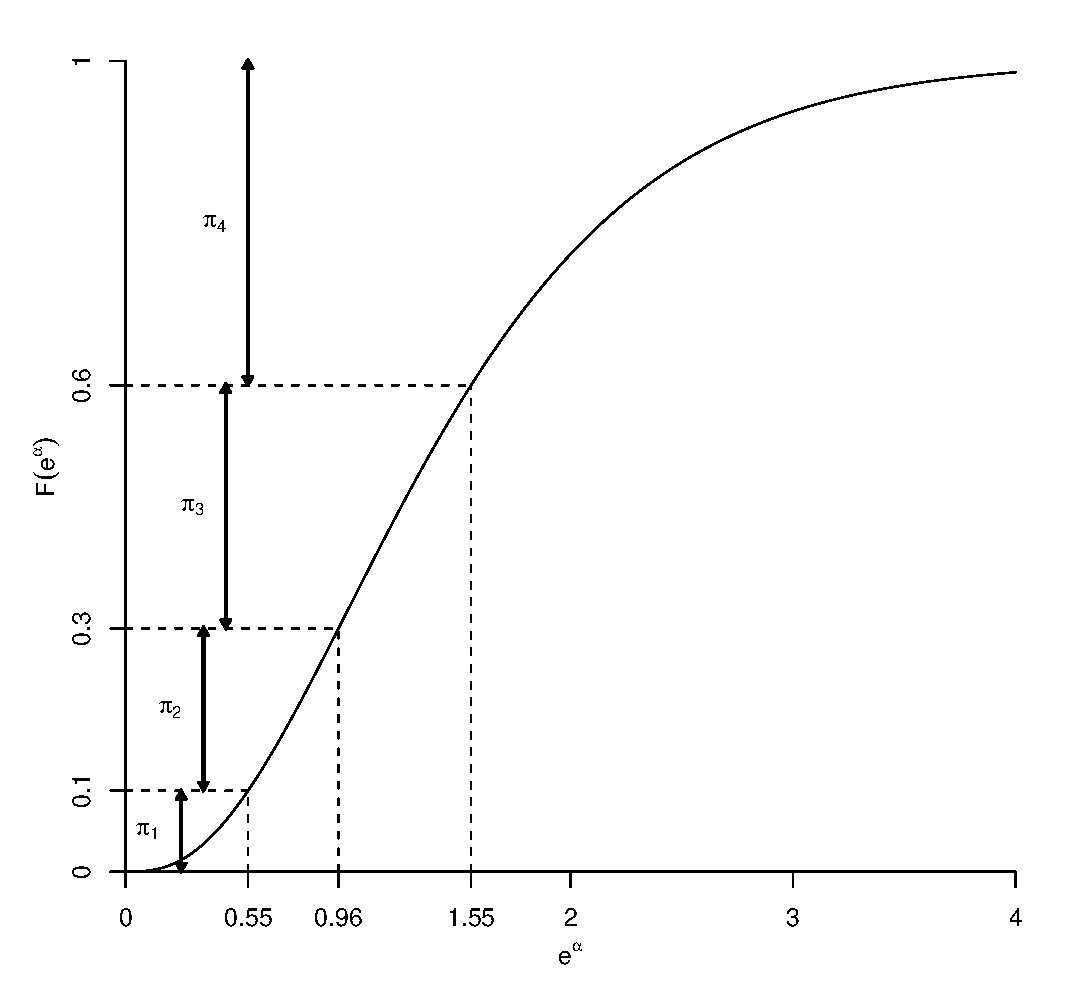
\includegraphics[width=4in]{mix/figs/pidia.pdf}
\caption{Illustration of the parameterisation of the $\pi_j$s. The black curve is a Gamma CDF (with shape parameter 3 and scale parameter 1/2). Here $\bm{\pi}=(0.1,0.2,0.3,0.4)$. The differences in the ``heights'' of the evaluations of the CDF give the values of $\pi_j$.}
\label{dlbpi}
\end{figure}

\subsubsection{Inverse transform}
\label{mmds-pi-inv}
To transform from the $\pi_j$s back to the $\alpha_j$s we simply re-arrange the above expression.
\begin{align*}
\pi_j &= F(\sum_{k=1}^j e^{\alpha_k}) - F(\sum_{k=1}^{j-1} e^{\alpha_k})\\
F(\sum_{k=1}^j e^{\alpha_k}) &= \pi_j + F(\sum_{k=1}^{j-1} e^{\alpha_k})\\
\sum_{k=1}^j e^{\alpha_k} &= F^{-1}(\pi_j + F(\sum_{k=1}^{j-1} e^{\alpha_k}))\\
e^{\alpha_j} &= F^{-1}\Big(\pi_j + F(\sum_{k=1}^{j-1} e^{\alpha_k})\Big) - \sum_{k=1}^{j-1} e^{\alpha_k}\\
\alpha_j &= \log_e \Big(F^{-1}\Big(\pi_j + F(\sum_{k=1}^{j-1} e^{\alpha_k})\Big) - \sum_{k=1}^{j-1} e^{\alpha_k}\Big)
\end{align*}
Thus, it is possible to move between $\pi_j$s and $\alpha_j$s easily.

\subsection{Fitting}
It is well known that mixture model likelihoods are notoriously multi-modal (\cite{BDA} PAGES).

(TKTKTK more here)

Three different strategies were used for the optimisation and offered in the \texttt{mmds} package. The justification being that if one method fails to fit a particular model, then perhaps another might be better at tackling that particular problem. The first and simplest of these methods is a straightforward quasi-Newton method, BFGS (\cite{bfgs}) which simply maximises the likelihood with the help of analytic gradients (see appendix \ref{appendix-mmds-derivs}). In testing this method was unsatisfactory so two other procedures were also developed.

\subsection{BFGS+SANN}
The starting value calculation (see section \ref{mmds-starting-vals}) is relatively primitive and therefore perhaps does not start the optimisation in a particularly good position to begin the maximisation. Given this and the rather complex likelihood, the odds are not stacked in the favour of the optimisation procedure being successful. In order to move around the parameter space, simulated annealing (\cite{numrec}, pp. 549--554) is used to begin the maximisation then followed by a BFGS round to find the maxima. Both BFGS and simulated annealing are available via the \texttt{optim()} function in the base \textsf{R} distribution.

In particular, simulated annealing is used for 250 iterations, then unconstrained BFGS after that. In an attempt to avoid local maxima, these two steps are looped for five iterations and the results stored. The model with the lowest AIC is then chosen from these. If no models fit in the first 5 iterations, the procedure continues until at least one model fits, or there have been 20 attempts at fitting, whichever comes first.

It is worth noting that the method may appear to fail to converge for all attempts, however this does not necessarily indicate that the model will never converge. The stochastic nature of simulated annealing means that it is entirely possible that further runs may yield a useful result.

\subsection{Expectation-Maximisation Algorithm}
A common (TKTKTK cite!) way of fitting mixture models is to use the Expectation-Maximisation (EM) algorithm of \cite{em}. (TKTKTK WHY?!)


\subsubsection{Overview}

(TKTKTK Re-write this)

Considering each of the observations as coming from one of the $J$ mixture components, we arrive at a latent variable interpretation of the mixture model. Given this latent variable view, it is possible to then evaluate the probability that each observation is from a particular mixture component. The mixture proportions can then we calculated by taking the expectation over the observations of these ``weights'' for a given mixture component. Once the mixture proportions are calculated, the scale parameters can be found using a some optimisation procedure (such as BFGS) keeping the mixture proportions constant within BFGS. This yields a new set of scale parameters, so the mixture proportions are then recalculated. EM switches between these two stages (expectation and maximisation) until the values for the mixture proportions and the scale parameters have converged.

\subsubsection{EM steps}
The expectation and maximisation steps are defined as follows. First note that $f_j(x_i;\sigma_j(\bm{z}_i,\bm{\beta}_j))$ is the PDF of mixture part $j$ evaluated at distance $x_i$ with covariates $\bm{z}_i$. 


\begin{itemize}
\item \textbf{Expectation.}
During the expectation step the mixture proportions are calculated. This is done using the expected values of the weights, $w_{ij}$, for each datum $i$ and mixture $j$,
\begin{equation*}
\mathbb{E}[w_{ij}] = \frac{\pi_j f_j(x_i;\sigma_j(\bm{z}_i,\bm{\beta}_j))}{\sum_{k=1}^J \pi_k f_k(x_i;\sigma_k(\bm{z}_i,\bm{\beta}_k))}.
\end{equation*}
Then $\pi_j$s may be calculated as:
\begin{equation*}
\pi_j=\frac{1}{n} \sum_{i=1}^n \mathbb{E}[w_{ij}].
\end{equation*}

\item \textbf{Maximisation.}
Keeping the $\pi_j$s fixed (from the previous step), optimise with respect to the $\sigma_j$s (or, rather, $\beta_{jk}$s). Here BFGS is used with analytic gradients (see appendix \ref{appendix-mmds-derivs}). 
\end{itemize}



cite EM/CEM/SEM paper

% maybe show why other parametrisation doesn't work??


\subsection{Starting values}
\label{mmds-starting-vals}
\cite{beavers98} give a method for estimating starting values for the scale parameter of a half-Normal detection function. In the non-covariate case, the estimate is given as the intercept parameter from intercept only regression on $\log(x+\frac{w}{1000})$ (where $w$ denotes the truncation distance, as above). For covariate models, the equation used for the $\sigma$ is used in the regression and the estimated parameters from the linear regression are used as the starting values for the $\beta$s.

A similar approach can be use in the mixture case by first sorting data by distance and then dividing it into $k$ equal parts (for a $k$ point mixture). For each of these parts a \cite{beavers98}-type estimate is used for the $\beta_{jk}$s (or $\beta_j$s in the non-covariate case).

For the $\alpha_j$s, a set of $\pi_j$ are generated as $1/k$ and then transformed by the procedure given in section \ref{mmds-pi-inv} to be on the $\alpha_j$ scale.


\subsection{Derivatives}

\textbf{SIMON}: I was going to do this as an appendix, since otherwise there's just a massive chunk of maths in the middle of this chapter.

%%%%%%%%%%%%%%%%%%%%%%%%%%%%%%%%%%%%%%%%%%%%%%%%%%%
\section{Testing}

The models detailed above were run on both real and simulated data to test their efficacy. Simulations of the most common models are presented first, followed by analyses of real data. The analyses of real data are available as a vignette written in Sweave (\cite{sweave}) at URL HERE.

\subsection{Simulations}

Four classes of models were tested, giving a range of easy and hard problems over possible sampling scenarios. The classes were:
\begin{itemize}
	\item Non-covariate 2-point mixtures for line transect data.
	\item Non-covariate mixtures for point transect data.
	\item Non-covariate 3-point mixtures for line transect data.
	\item Covariate mixtures for line transect data.
\end{itemize}
In order to assess how well the models performed, two metrics were used. The first metric is parameter estimates returned from the optimisation procedure -- this should highlight that the optimisation is working numerically and can successfully recover the parameters. The second metric is the abundance estimate ($\hat{N}$). The latter measure may be important as changes in the parameters may give (approximately) equal values of $\hat{N}$, since the parameter estimates are not usually of interest (the ultimate output being the abundance or density estimate in a distance sampling analysis), it makes sense to look at $\hat{N}$.

For each set of parameters for each of the model classes, 500 realisations were generated at each of 5 sample sizes (30, 60, 120, 480, 960). Samples were drawn, according to their proportions from the appropriate half-normal distributions using the \texttt{rtnorm()} function in the \texttt{msm} package in \textsf{R}. Where the proportions did not provide integer divisions of the sample sizes residual sampling (TKTKTK cite Baker 1985) was used. The truncation distance in each case was set to 1 in all cases and the parameters selected such that $g(1)\approx 0.15$.

\subsubsection{Non-covariate 2-point mixtures for line transect data}

Five parameter combinations were used to test non-covariate 2-point mixtures the parameters are given in table \ref{mmds-nocov-simtable} (in the more human-readable $\sigma$ and $\pi$ parametrisation) and their corresponding detection functions are plotted in figure \ref{mmds-nocov-funcs}.

\begin{table}[ht]
\centering
\begin{tabular}{c c c c}
Sim no. & $\sigma_1$ & $\sigma_2$ & $\pi_1$\\
\hline
\hline
1 & 0.2 & 0.8 &  0.36\\
2 & 0.8 & 0.2 & 0.44\\
3 & 0.2 & 0.8 & 0.18\\
4 & 10  & 0.2 & 0.44\\
5 & 0.01&  0.8 & 0.29\\
\end{tabular}
\label{mmds-nocov-simtable}
\caption{Simulation parameters for the non-covariate simulations. (In $\sigma$ and $\pi$ parametrisation).}
\end{table}

The first three simulations give relatively simple scenarios with the same scale parameters but varying the mixture proportions, these check behaviour under ``easy'' conditions. The fourth checks to see what happens when one of the mixtures is essentially too big to be identified (it starts to decrease after the truncation distance so the parameter value could be 10, 100 or even 1000). Finally the fifth example gives and extremely spiked detection function.

% detection functions for nocov
\begin{figure}
\centering
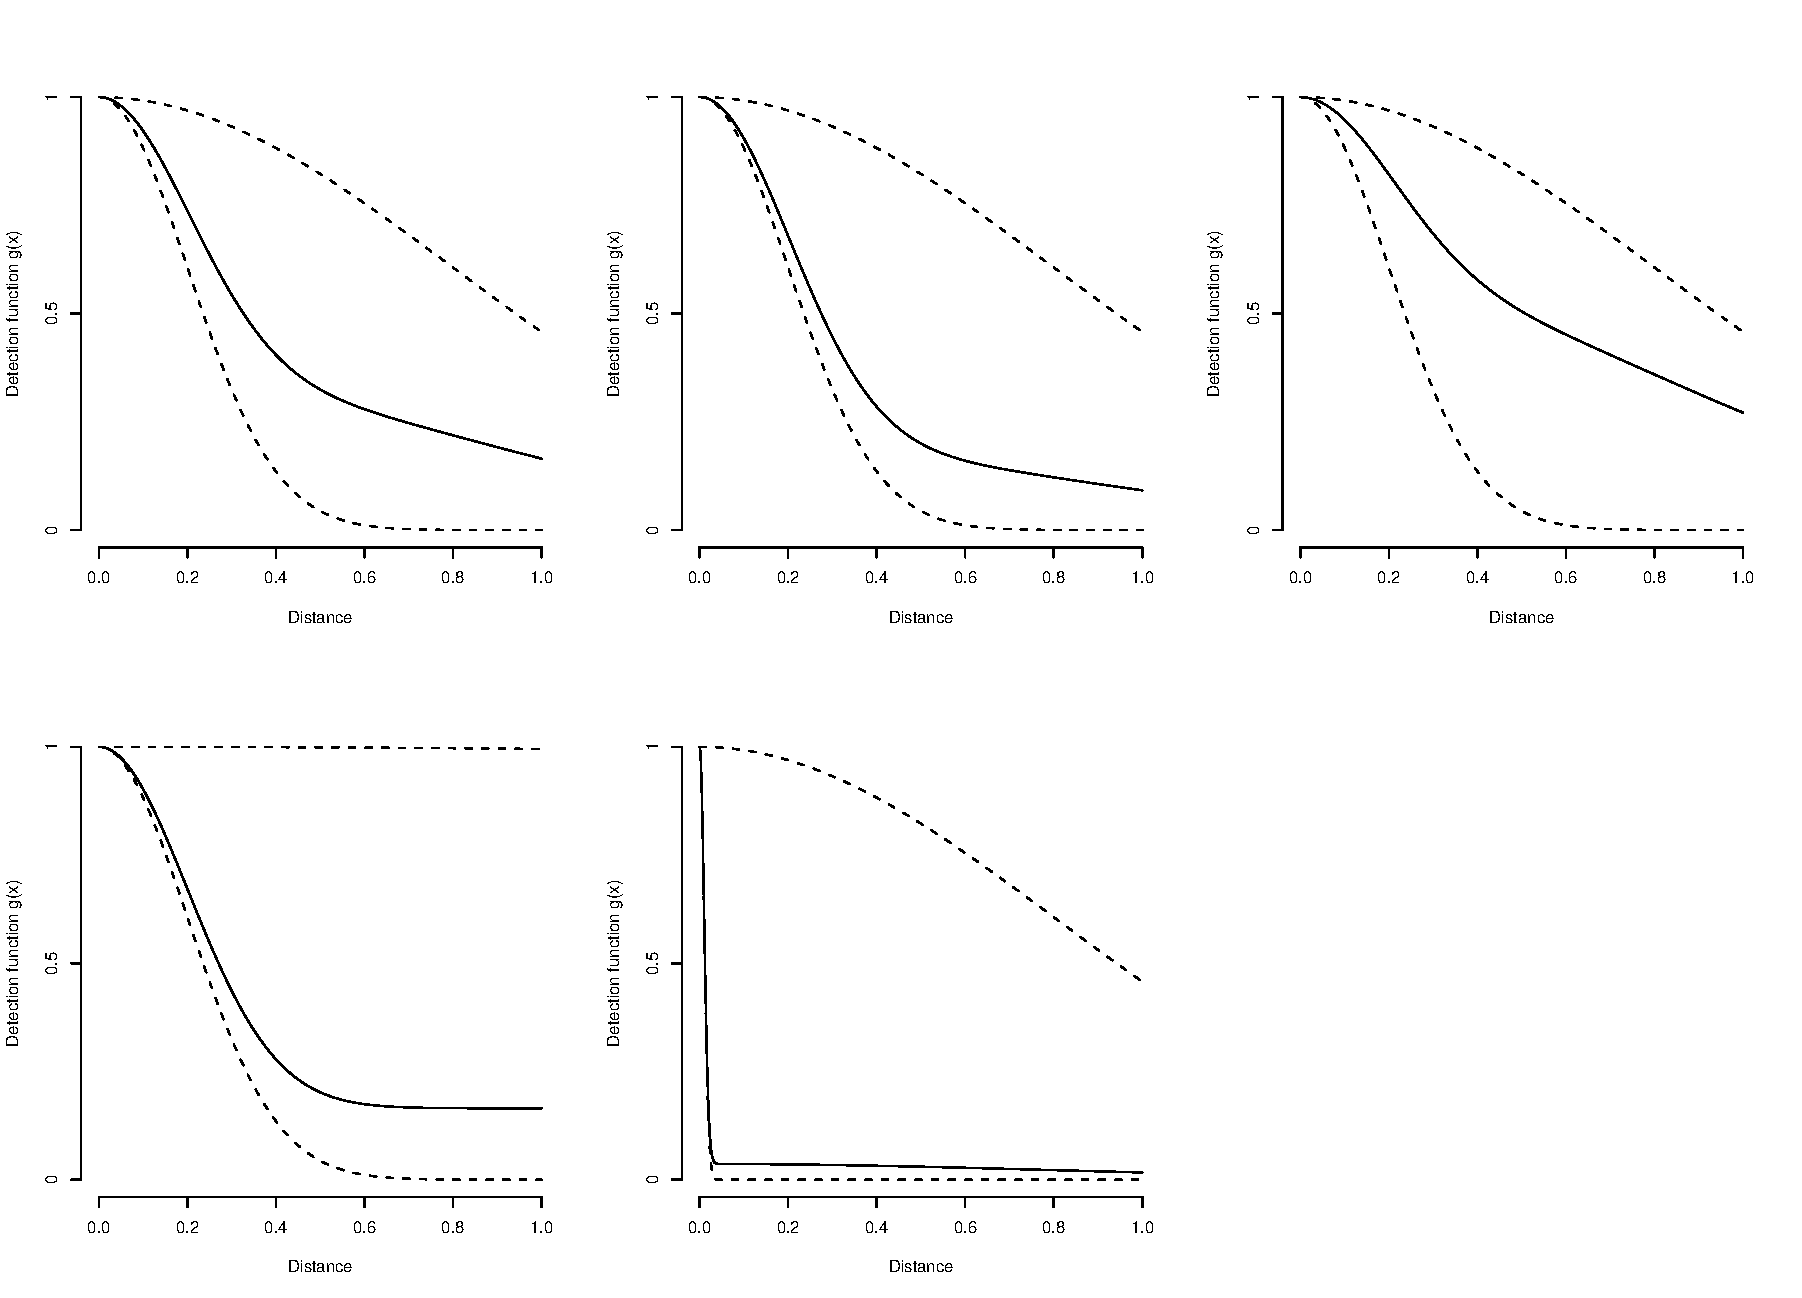
\includegraphics[width=6in]{mix/figs/nocovsims.pdf}
\caption{Detection functions used for the non-covariate 2-point mixture simulations for line transects.}
\label{mmds-nocov-funcs}
\end{figure}

TKTKTK
Figure \ref{mmds-nocov-boxplots} shows boxplots of the parameter estimates (for $\sigma_1$, $\sigma_2$, $\pi_1$ and $\pi_2$, top to bottom) for scenarios 1 through 5 (left to right), the boxes are colour coded according to the optimisation method. The first three scenarios show a rather nice pattern, gradually getting closer to the truth with less uncertainty as the sample size increases. Scenarios 4 and 5 however deserve more attention.

% big boxplots of par estimates
\begin{figure}
\centering
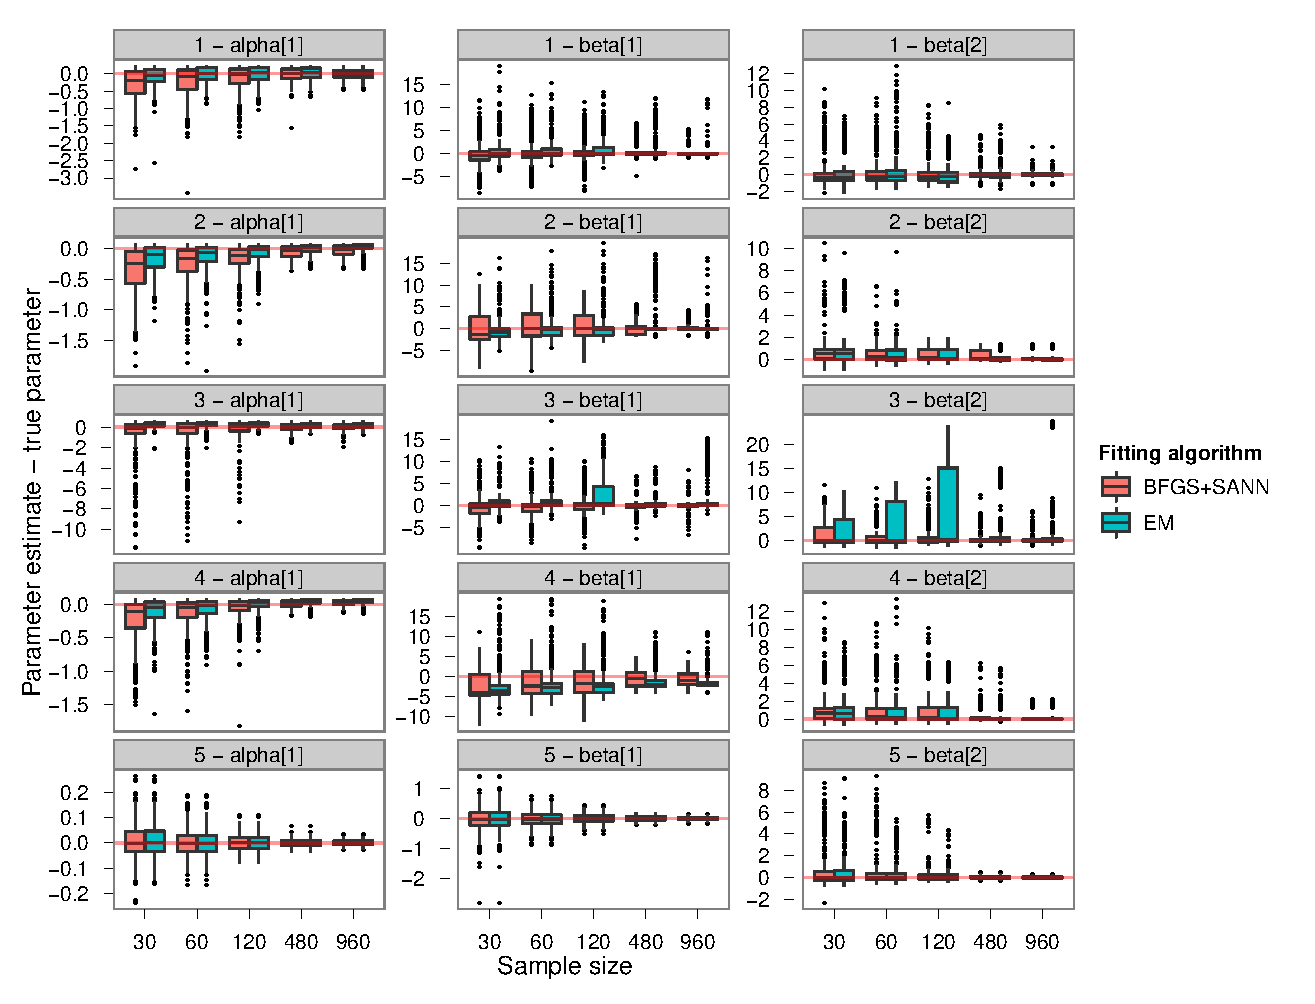
\includegraphics[width=7in]{mix/figs/nocov-boxplots.pdf}
\caption{TKTKTK WRONG ORDER!!!! [[change labels, large scale par-small scale par?]]}
\label{mmds-nocov-boxplots}
\end{figure}
% generated by mmds/paper/code/papersims/nocov/analyse.R

% boxplots of N
\begin{figure}
\centering
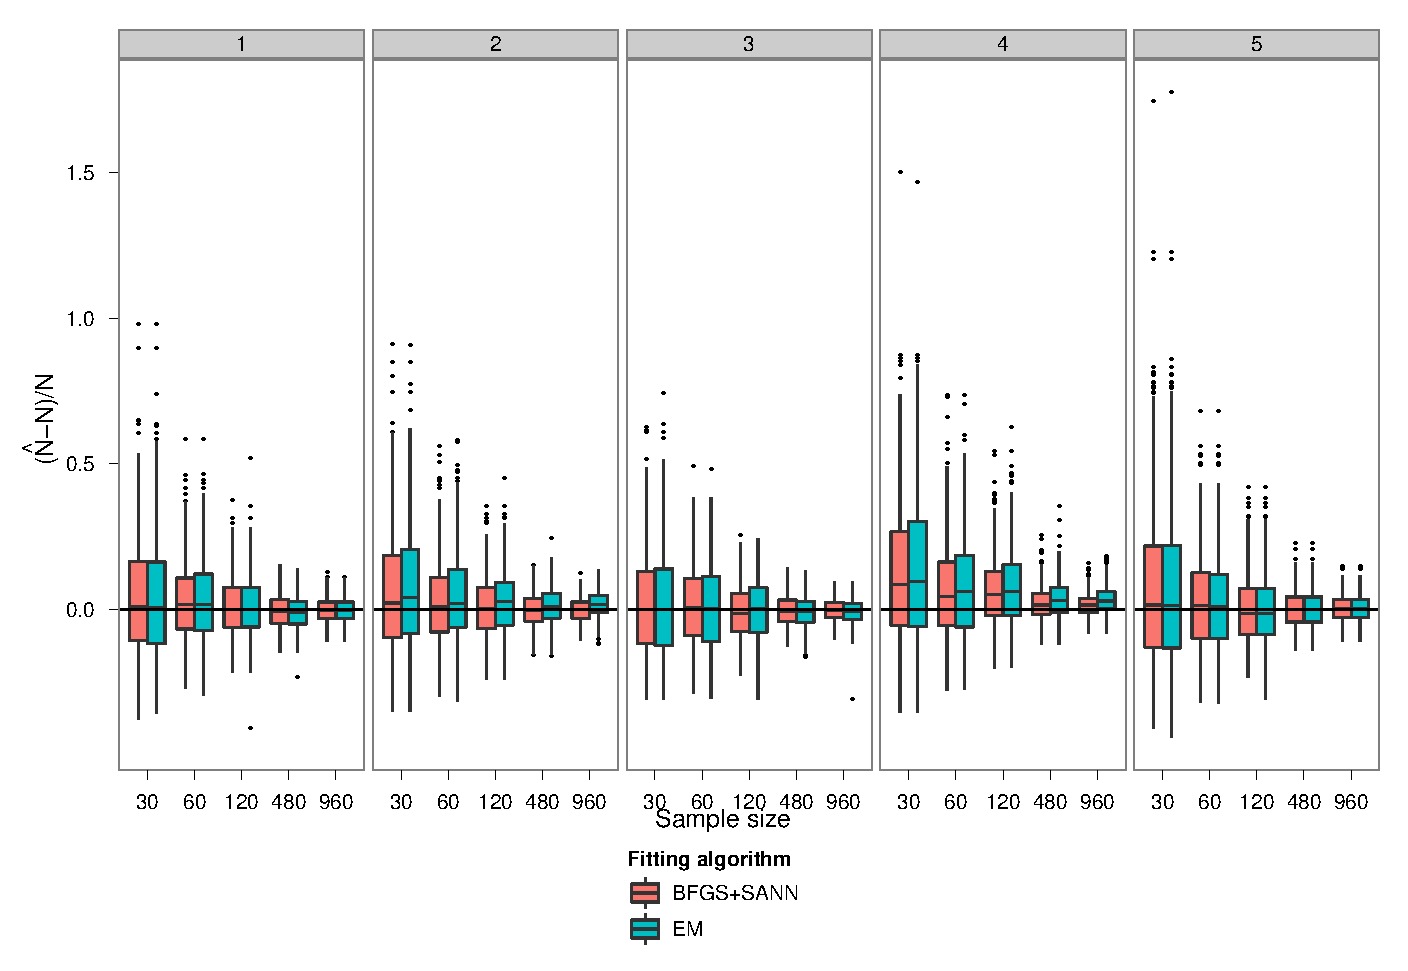
\includegraphics[width=6in]{mix/figs/nocov-N.pdf}
\caption{Boxplots of the estimated abundance for each of the simulations with colour-coded fitting method. TKTKTK}
\label{mmds-nocov-N-boxplots}
\end{figure}
% generated by mmds/paper/code/papersims/nocov/analyse-pa.R

Scenario 4 was deliberately set up to see if, when one of the parameters is unidentifiable, the estimates of $P_a$ are incorrect. Figure \ref{mmds-nocov-pa-boxplots} shows that they do not appear to suffer. However, looking at figure \ref{mmds-nocov-boxplots} we see that there is a large amount of variability in the parameter estimates even though the estimates of average detectability are correct. This is to be expected given that there is very little information available on the scale parameter, aside from the fact that it is ``big''. Even though this is a rather tough case, the estimates of average detectability are reliable. 

Scenario 5 consists of one spiked function and one wide function, the mixture proportion is (0.29,0.71). As such about 30\% of the observations lie in the spike and 70\% in the wider function; since there is such a large difference in the two functions, the model is actually easier to fit that the others. When the sample size is low, there are many outliers, however when the optimisation does not go catastrophically wrong, it tends to do very well, as can be seen from the low variability. This probably indicates that there is a well defined maxima in the likelihood.

(TKTKTK Put in some of the extra plots here and discuss?)


Table \ref{mmds-nocov-pa-table} shows the mean squared error and bias in the estimates of $P_a$ for each of the fitting methods. Note that there is not a particularly big difference between the methods, as can be seen in figures \ref{mmds-nocov-boxplots} and \ref{mmds-nocov-pa-boxplots}.



\subsubsection{Non-covariate 3-point mixtures for line transect data}

Two scenarios were used to test 3-point mixtures. The parameters are given in table [PAR TABLE] and the corresponding detection functions are given in figure [DETFCT FIG]. Data was generated from these models in the same manner as above and both 3-point and 2-point mixture models were fit. It is possible that 2-point mixtures may be flexible enough in most situations that 3-point mixtures are not necessary. Simulating data from a model that truly a 3-point mixture and fitting a 2-point mixture to it should highlight if this is the case.


TKTKTK [[ PAR TABLE HERE]]

TKTKTK [[DETFCT FIG HERE]]

TKTKTK [[ looks like the 3rd par is really big. Is this because it wants to fit a 2-point mixture instead? ]]

TKTKTK [[ does very badly on the sigma=15 par, this par has pi=0.1, so do the pis matter more than the sigmas? --- maybe, this is what seems to be indicated in 2 point case, but need to look into it more]]



\subsubsection{Covariate 2-point mixtures for line transect data}

Two models were used to test covariate 2-point mixtures. In both cases the models had scale parameters obeying:
\begin{equation}
\sigma_{i1} = \exp(\beta_{10}+z_{i1} \beta_1),\\
\sigma_{i2} = \exp(\beta_{20}+z_{i1} \beta_1).
\end{equation}
In one model $z_i1$ was a dichotomous factor variable and in the other $z_i1$ was a continuous variable ...


\subsubsection{Non-covariate 2-point mixtures for point transect data}


WHY are we doing each of these.

DISCUSSION OF (in particular)



covar with 3pt - what's going on?

3pt with 2pt - what's going on





\subsection{Real data}

Just source in the .tex from the vignette?




%%%%%%%%%%%%%%%%%%%%%%%%%%%%%%%%%%%%%%%%%%%%%%%%%%%
\section{Conclusion}


%\section{Acknowledgements}
%
%I would like to thank David Borchers for his comments on my MMath thesis, on which this work was based, as well as the parametrisation for the mixture proportions. I would also like to thank Jeff Laake and Steve Buckland for interesting discussions about the topic. Finally I would like to thank Len Thomas my co-author.
%
%Outline of the EM algorithm is taken from the very helpful set of notes by \cite{piater}.

